\documentclass[a4paper, 12pt, onecolumn, twoside]{article}

\usepackage[utf8]{inputenc}
\usepackage{amsmath}
\usepackage{amssymb}
\usepackage{graphicx}
\usepackage[hidelinks]{hyperref}
\usepackage{float}
\usepackage{enumitem}



\title{%
  Resumos de AC2 \\
  \large Teste Teorico 2}

\author{Tiago Almeida}
\date{\today}

\begin{document}

\maketitle

\tableofcontents

\section{Introdução}
Escrever um pequeno overview da matéria que sai para o teste teórico 2
e o que esperar encontrar neste documento

\clearpage

\section{A Interface \hyperref[spi]{\textbf{\large{SPI}}}}
\hyperref[spi]{\textbf{SPI}} é uma interface de \textbf{alta velocidade e de curta distância} (dezenas de cm) usada para comunicar com
diversos dispositivos diferentes, como por exemplo:
\begin{itemize}
    \item Sensores de diversos tipos: temperatura, pressão, etc.
    \item Cartões de memória (MMC / SD)
    \item Circuitos: memórias, ADCs, DACs, Displays LCD (e.g.\ telemóveis),
    comunicação entre corpo de máquinas fotográficas e as lentes, \ldots
    \item Comunicação entre microcontroladores
\end{itemize}

A transferencia de dados em \hyperref[spi]{\textbf{SPI}} é ciclica, isto é, tudo o que é enviado é recebido de volta por quem enviou.
Assim, existem 3 tipos de transferência possiveis:
\begin{itemize}
    \item \textbf{Bidirecional}: são transferidos dados válidos em ambos os sentidos
    (master → slave e slave → master)
    \item \textbf{Master → slave (operação de escrita)}: master transfere dados
    para o slave, e ignora/descarta os dados recebidos
    \item \textbf{Slave → master (operação de leitura)}: master pretende ler dados do slave; 
    para isso transfere para o slave uma palavra com informação irrelevante (por exemplo 0); 
    o slave ignora/descarta os dados recebidos
\end{itemize}
\subsection{Funcionamento}
Pontos chave sobre a arquitetura do \hyperref[spi]{\textbf{SPI}}:\@
\begin{itemize}
    \item Apenas tem \textbf{1 master} mas pode ter \textbf{1 ou mais slaves}
    \item Relógio gerado e controlado pelo master
    \item Comunicação síncrona
    \item Comunicação \hyperref[fullduplex]{full-duplex}
    \item Apenas 1 slave pode ser selecionado por vez através do sinal \hyperref[ss]{SS}
    \item O master inicia e controla a transferência de dados, com a sinalização:
    \begin{itemize}
        \item \hyperref[sck]{\large\textbf{{SCK}}}: clock
        \item \hyperref[mosi]{\large\textbf{{MOSI}}}: Master Output Slave Input (SDO no
        master)
        \item \hyperref[miso]{\large\textbf{{MISO}}}: Master Input Slave Output (SDI no
        master)
        \item \hyperref[ss]{\large\textbf{{SS}}}: Slave select
    \end{itemize} 
    \item Quando o master envia um byte, o slave tambem envia um byte de volta ao mesmo tempo.
    Isso ocorre porque o SPI usa shift registers circulares para transferir dados.
    \begin{figure}[h]
        \centering
        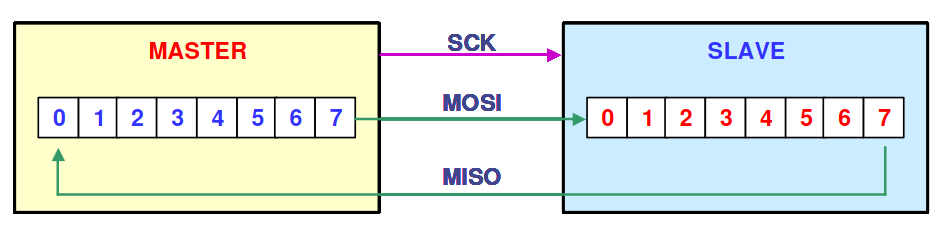
\includegraphics[width=1\textwidth]{Funcionamento_SPI.png}
        \caption{Exemplo do funcionamento do SPI}\label{fig1}
    \end{figure}
    \item Dados relevantes e Inúteis:
    \begin{itemize}
        \item Os dados que o slave envia de volta podem ou não ter significado. Se o slave não tiver dados 
        relevantes para enviar, ele pode enviar bytes preenchidos com zeros, valores padrão ou dados que não 
        são importantes para o contexto da comunicação.
    \end{itemize}
    \item Protocolo e Significado dos Dados:
    \begin{itemize}
        \item O significado dos dados trocados entre master e slave depende do protocolo de comunicação específico 
        implementado no software. O master e o slave devem ter um acordo prévio sobre o que os dados representam e 
        como devem ser interpretados.
    \end{itemize}
\end{itemize}

\clearpage
\subsection{Arquiteturas de ligação}

No caso do SPI, existem 2 arquiteturas de ligação:
\begin{itemize}
    \item \textbf{Slaves independentes}
    \item \textbf{Daisy chain}
\end{itemize}
\begin{figure}[H]
    \centering
    \begin{minipage}{0.48\textwidth}
        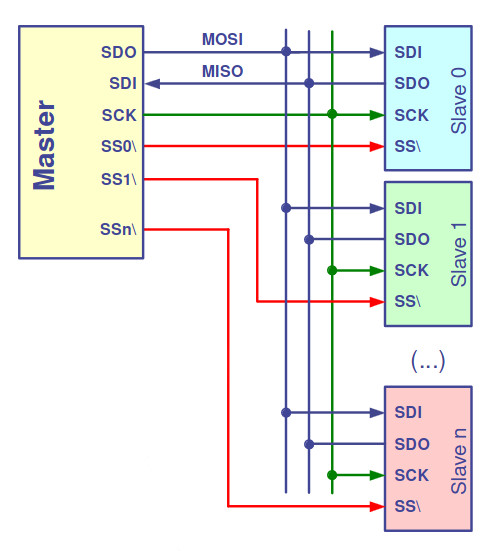
\includegraphics[width=\textwidth]{Arquitetura-de-ligação-1_SPI.jpg}
        \caption{Exemplo da arquitetura `Slaves independentes' do SPI}\label{fig2}
    \end{minipage}
    \hfill
    \begin{minipage}{0.48\textwidth}\label{fig3}
        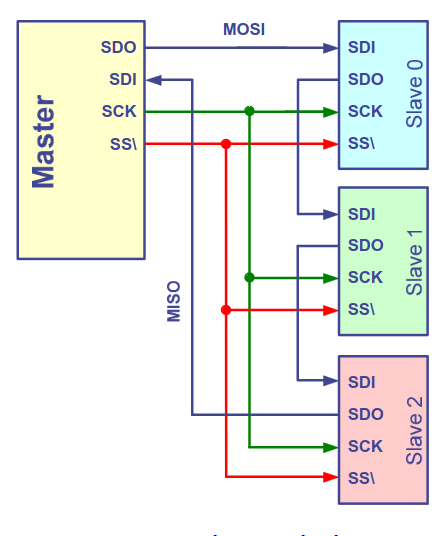
\includegraphics[width=\textwidth]{Arquitetura-de-ligação-2_SPI.png}
        \caption{Exemplo da arquitetura `Daisy chain' do SPI}
    \end{minipage}
\end{figure}

No primeiro tipo, Slaves independentes, existe no master um sinal de seleção, 
sinal \hyperref[ss]{SS} individual para cada salve.
\begin{itemize}
    \item Apenas um sinal \hyperref[ss]{SSx} pode estar ligado de cada vez
    \item O número maximo de slaves está limitado pelo numero de \hyperref[ss]{SS}
    \item O microcontrolador pode gerar, através dos seus portos digitais, sinais \hyperref[ss]{SSx} de forma a ultrapassar a limitação anterior  
\end{itemize}

\clearpage
No segundo tipo, Daisy chain, existe no master um unico sinal hyperref[ss]{SS} common para todos os slaves.

\begin{itemize}
    \item Como podemos ver pelo fio azul do \hyperref[fig3]{exemplo de daisy chain}, a informação tem de passar
    por todos os slaves até voltar ao master, logo os slaves tem de ter a capacidade de armazenar uma sequência de N bits.
    \item Enquando o \hyperref[ss]{SS} estiver ativo, o slave ignora o comando recebido e envia para o slave seguinte ou para o master no caso do ultimo slave.
    \item O slave apenas executa o comando quando o sinal \hyperref[ss]{SS} for desativado
\end{itemize}




\subsection{Detalhes adicionais}
Algumas notas adicionais sobre \hyperref[spi]{\textbf{SPI}} que podem ou não ser importantes:

\begin{itemize}
    \item Criado pela empresa Motorola
    \item Não é exigido precisão no relógio. 
    \begin{itemize}
        \item Permite com que o se possa optar por um oscilador de baixo custo 
        \item Não é necessário um cristal de quartzo
    \end{itemize}
    \item Facil de implementar por hardware ou por software
    \item O SPI funciona sempre em modo `data exchange', isto é, o processo de comunicação 
    envolve sempre a troca do conteúdo dos shift-registers do master e do slave. 
    Cabe aos dispositivos envolvidos na comunicação usar ou descarta a informação recebida
    \item 
\end{itemize}

\section{Conclusão}
Algumas conclusões e considerações que se deve ter após
ter acabado o estudo

\clearpage
\section{Glossário}\label{glossary}

Aqui está a secção de glossário. Cada termo usado repetidamente no documento está listado aqui com sua definição.

\begin{itemize}
    \item\label{spi} \textbf{SPI}: Serial Peripheral Interface
    \item\label{simplex} \textbf{Simplex}: comunicação apenas num sentido (TX -> RX); usada, por
    exemplo, em telemetria, para leitura remota de sensores
    \item\label{halfduplex} \textbf{Half-Duplex}: comunicação nos dois sentidos, mas apenas um de
    cada vez (é usada uma só linha)
    \item\label{fullduplex} \textbf{Full-Duplex}: Comunicação simultânea nos dois sentidos (são
    usadas duas linhas)
    \item\label{ss} \textbf{SS}: Slave select. Sinal usado pelo master para selecionar o slave. Por vezes
    tambem é usado CS (chip select) como selecionador de slave.
    \item\label{sck} \textbf{SCK}: Clock. Relógio gerado pelo master que sincroniza a transmissão/receção de dados
    \item\label{mosi} \textbf{MOSI}: Master Output Slave Input (SDO no master).
    Linha do master para envio de dados para o slave
    \item\label{miso} \textbf{MISO}: Master Input Slave Output (SDI no master).
    Linha do slave para enviar dados para o master
\end{itemize}

\end{document}
